\documentclass[a4paper]{article}
\usepackage[a4paper,margin=0mm]{geometry}
\usepackage{fontspec}
\usepackage{unicode-math}
\usepackage{tikz}
\usetikzlibrary{fit,calc,positioning}
\usepackage[table]{xcolor}
\usepackage[absolute]{textpos}
\usepackage{array}

\setmainfont{Libertinus Serif}
\setsansfont{Libertinus Sans}
\setmathfont{Libertinus Math}

\definecolor{accent}{HTML}{F46530}
\definecolor{badge}{HTML}{FFBDA5}
\definecolor{ink}{HTML}{2A2E30}

\setlength{\TPHorizModule}{1mm}
\setlength{\TPVertModule}{1mm}
\setlength{\parindent}{0pt}
\pagestyle{empty}

\newcommand{\topicheader}[2]{%
\begin{textblock*}{194mm}(16mm,10mm)
\begin{tikzpicture}
\node[fill=accent,text=white,font=\sffamily\bfseries\fontsize{13}{13}\selectfont,
      minimum width=9mm,minimum height=9mm,inner sep=0pt] at (4.5mm,-4.5mm) {#1};
\node[font=\sffamily\bfseries\fontsize{15}{16}\selectfont,text=ink,anchor=west] at (12mm,-4.5mm) {#2};
\end{tikzpicture}
\end{textblock*}
\begin{textblock*}{194mm}(16mm,22.5mm)

\begin{tikzpicture}
\fill[accent] (0,0) rectangle (194mm,0.5mm);
\end{tikzpicture}
\end{textblock*}
}

\newcommand{\pagekicker}[1]{%
\begin{textblock*}{100mm}(16mm,25.5mm)
\begin{tikzpicture}
\node[fill=ink,text=white,font=\sffamily\bfseries\fontsize{8}{8}\selectfont,
      inner sep=2.2pt,rounded corners=1pt] {\MakeUppercase{#1}};
\end{tikzpicture}
\end{textblock*}
}

\newcommand{\pagefooter}[1]{%
\begin{textblock*}{194mm}(8mm,286.41mm)
  
\begin{tikzpicture}
    \fill[accent] (0,0) rectangle (194mm,0.6mm);
  \end{tikzpicture}
\end{textblock*}
\begin{textblock*}{63.59mm}(8mm,288.27mm)
  {\sffamily\bfseries\color{accent}\fontsize{13}{16}\selectfont SAT 1200+}
\end{textblock*}
\begin{textblock*}{10mm}(188mm,288.27mm)
  \centering{\sffamily\color{accent}\fontsize{14}{16}\selectfont #1}
\end{textblock*}
}

\newcommand{\cardbg}[4]{%
\begin{textblock*}{#3mm}(#1mm,#2mm)
\begin{tikzpicture}
\fill[badge!22,rounded corners=3mm] (0,0) rectangle (#3mm,-#4mm);
\end{tikzpicture}
\end{textblock*}%
}

\newcommand{\pill}[3]{%
\begin{textblock*}{160mm}(#1mm,#2mm)
\begin{tikzpicture}
\node[fill=accent,text=white,anchor=north west,font=\sffamily\bfseries\fontsize{10}{10}\selectfont,
      rounded corners=8pt,inner xsep=5mm,inner ysep=1.8mm] at (0,0) {QOIDA ~\textperiodcentered~ #3};
\end{tikzpicture}
\end{textblock*}%
}

\arrayrulecolor{accent}
\setlength{\arrayrulewidth}{0.7pt}
\renewcommand{\arraystretch}{1.5}

\begin{document}

\topicheader{2}{Kasrlar}
\pagekicker{Formula sheet}
\pagefooter{14}
\mbox{}%

% ================= CARD 1: Surat, maxraj, soddalashtirish (y: 33-83) =================
\cardbg{16}{33}{178}{50}
\pill{26}{36}{Surat, maxraj, soddalashtirish}

\begin{textblock*}{158mm}(26mm,49mm)
\begin{tikzpicture}
\node[font=\fontsize{11}{11}\selectfont,text=accent] (surat) at (0,10mm) {surat};
\node[font=\fontsize{20}{20}\selectfont] (frac) at (28mm,0) {$\dfrac{24}{36}$};
\node[font=\fontsize{11}{11}\selectfont,text=accent] (maxraj) at (0,-10mm) {maxraj};
\draw[accent,->,line width=0.8pt] (surat.east) -- ++(10mm,-4mm);
\draw[accent,->,line width=0.8pt] (maxraj.east) -- ++(10mm,4mm);

\node[font=\fontsize{20}{20}\selectfont] at (70mm,0) {$\xrightarrow{\ \div\,12\ }$};
\node[font=\fontsize{20}{20}\selectfont,text=accent] at (95mm,0) {$\dfrac{2}{3}$};
\node[font=\sffamily\fontsize{9}{10}\selectfont,text=black!55] at (95mm,-13mm) {eng oddiy ko'rinish};
\end{tikzpicture}
\end{textblock*}

% ================= CARD 2: Qo'shish / Ayirish (y: 89-164) =================
\cardbg{16}{89}{178}{75}
\pill{26}{92}{Qo'shish / ayirish}

\begin{textblock*}{158mm}(26mm,103mm)
{\fontsize{11}{14}\selectfont\color{ink}
Maxrajlar har xil bo'lsa, avval umumiy maxrajga keltiring -- faqat shundan keyin suratlarni qo'shing yoki ayiring:}
\end{textblock*}

\begin{textblock*}{158mm}(26mm,116mm)
\begin{tikzpicture}[every node/.style={font=\fontsize{15}{15}\selectfont}]
\node[anchor=west] (l0) at (0,0) {$\dfrac{1}{4}+\dfrac{1}{6}$};
\node[anchor=west,font=\sffamily\bfseries\scriptsize,text=accent] at (60mm,0) {$\leftarrow$ 1. EKUK(4,6){=}12};

\node[anchor=west] (l1) at (0,-18mm) {$\dfrac{3}{12}+\dfrac{2}{12}$};
\node[anchor=west,font=\sffamily\bfseries\scriptsize,text=accent] at (60mm,-18mm) {$\leftarrow$ 2. suratlarni qo'shing};

\node[anchor=west,font=\sffamily\bfseries\fontsize{16}{16}\selectfont,text=accent] (l2) at (0,-36mm) {$=\dfrac{5}{12}$};

\foreach \y in {-5,-23}{
  \draw[accent,->,line width=1pt] (6mm,\y mm) -- (6mm,\y mm -6mm);
}
\end{tikzpicture}
\end{textblock*}

% ================= CARD 3: Ko'paytirish (left) / Bo'lish (right) (y: 170-225) =================
\cardbg{16}{170}{85}{55}
\pill{22}{173}{Ko'paytirish}

\begin{textblock*}{85mm}(16mm,188mm)
\begin{center}
{\fontsize{13}{13}\selectfont $\dfrac{4}{9}\times\dfrac{3}{8}$}

\vspace{2mm}
{\fontsize{10}{10}\selectfont\color{black!60} qisqartiring: $4\&8\to\div4$,\ \ $3\&9\to\div3$}

\vspace{2mm}
{\fontsize{14}{14}\selectfont\color{accent} $=\dfrac{1}{3}\times\dfrac{1}{2}=\dfrac{1}{6}$}
\end{center}
\end{textblock*}

\cardbg{109}{170}{85}{55}
\pill{115}{173}{Bo'lish}

\begin{textblock*}{85mm}(109mm,188mm)
\begin{center}
{\fontsize{13}{13}\selectfont $\dfrac{3}{4}\div\dfrac{2}{5}$}

\vspace{2mm}
{\fontsize{10}{10}\selectfont\color{black!60} teskarisiga ko'paytiring (K-C-F)}

\vspace{2mm}
{\fontsize{14}{14}\selectfont\color{accent} $=\dfrac{3}{4}\times\dfrac{5}{2}=\dfrac{15}{8}$}
\end{center}
\end{textblock*}

% ================= CARD 4: Aralash son <-> Noto'g'ri kasr (y: 231-281) =================
\cardbg{16}{231}{178}{50}
\pill{26}{234}{Aralash son $\leftrightarrow$ noto'g'ri kasr}

\begin{textblock*}{158mm}(26mm,249mm)
\begin{tikzpicture}
\node[font=\fontsize{15}{15}\selectfont] at (0,0) {$3\tfrac{2}{5}$};
\node[font=\fontsize{13}{13}\selectfont] at (24mm,0) {$\xrightarrow{\ 3\times5+2\ }$};
\node[font=\fontsize{15}{15}\selectfont,text=accent] at (52mm,0) {$\dfrac{17}{5}$};

\node[font=\fontsize{15}{15}\selectfont] at (90mm,0) {$\dfrac{23}{6}$};
\node[font=\fontsize{13}{13}\selectfont] at (116mm,0) {$\xrightarrow{\ 23\div6\ }$};
\node[font=\fontsize{15}{15}\selectfont,text=accent] at (144mm,0) {$3\tfrac{5}{6}$};
\end{tikzpicture}
\end{textblock*}

\begin{textblock*}{158mm}(26mm,262mm)
{\fontsize{9}{11}\selectfont\color{black!55}\itshape Butun son maxrajga ko'paytiriladi, suratga qo'shiladi -- maxraj o'zgarmaydi. Teskarisida: suratni maxrajga bo'ling, bo'linma -- butun son, qoldiq -- yangi surat.}
\end{textblock*}

\end{document}
